Androsec's dataset was created in two primary phases: The data collection and the static analysis phases. An overview of the collection and analysis process is shown in Figure~\ref{fig:ap}.

\begin{figure}[tbph]
\centering
\vspace{-0.2cm}
% 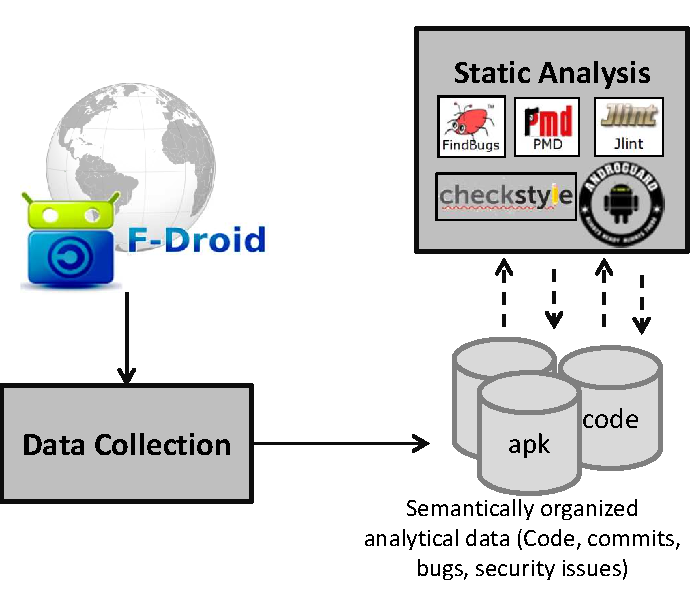
\includegraphics[width=0.9\linewidth]{./images/img}
%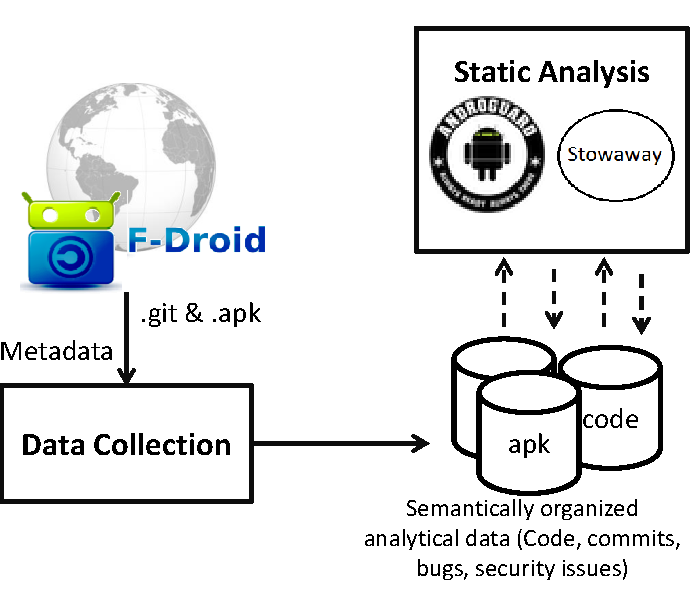
\includegraphics[scale=.6]{./images/collectionprocess.pdf}
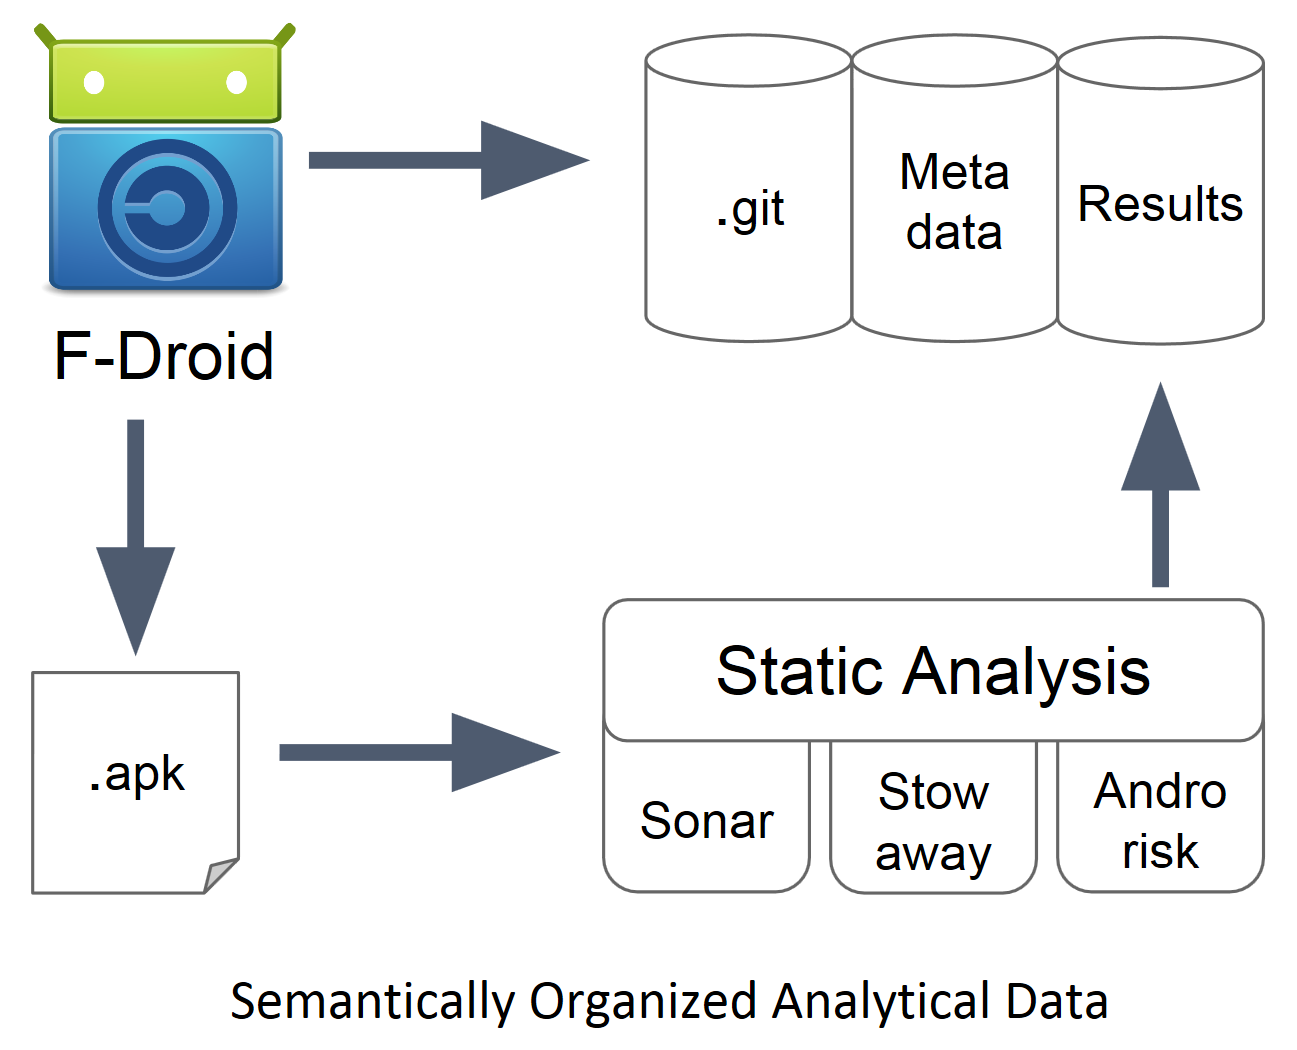
\includegraphics[scale=.18]{./images/process.png}


\caption{Collection \& Analysis Process\todo{make into latex?}}
\vspace{-0.2cm}
\label{fig:ap}
\end{figure}

\subsection{Collection}
%%% This is directly from the MSR paper
In the first phase we built a scraper tool to collect data from the F-Droid repository, extracting information from each app such as meta-data (name, description, and version), the source code of each major version, and its most recent apk (Android application) file. We collected version control information such as the committer's user name, commit time, and commit messages, ensuring all data was tagged with the version number to allow analysis over time. \dan{Add to this?}


\subsection{Analysis}
%%% Most of this text was taken directly from the MSR paper
Once collection was complete, we continued with analysis, running a variety of static analysis tools on the app's source code. Androrisk and Stowaway~\cite{Felt:2011:APD:2046707.2046779} were used to analyze the apk files, and Sonar was used on the extracted source code.\\

\textbf{Stowaway:} Android developers operate under a permission-based system where apps must be granted access (by the user and operating system) to various areas of functionality before they may be used. Examples include GPS location information, contacts, or the ability to make a phone call. If an app attempts to perform an operation to which it does not have permission, a~\emph{SecurityException} is thrown. Stowaway discovers these permission-gaps --- the over-permission and under-permission rate of an application.

Stowaway is comprised of two parts - API calls made by the app are determined using a static analysis tool and the permissions needed for each API are determined using a permissions map. In this study, we use the term \emph{over-permission} to describe a permission setting that grants more than what a developer needs for the task. Likewise, an \emph{under-permission} is a setting for which the app could fail because it was not given the proper permissions. Over-permissions are considered security risks and under-permissions are considered quality risks.

We selected Stowaway because it is able to state explicitly what over-permissions and under-permissions are present using a static-analysis based approach (not requiring an Android device or emulator). Stowaway has also demonstrated its effectiveness in existing research~\cite{Felt:2011:APD:2046707.2046779}. % Permlyzer~\cite{6698893}, a more modern permission detection tool, was not used because its authors have not made it available for download.


\textbf{Androrisk:} A component of the Androguard reverse engineering tool, Androrisk determines the security risk level of an application by examining several criteria. The first set is the presence of permissions which are deemed to be more dangerous. These include the ability to access the internet, manipulate SMS messages or the ability to make a payment. The second is the presence of more dangerous sets of functionality in the app including a shared library, use of cryptographic functions, and the presence of the reflection API.
 The total reported security risk score for each application is recorded and available.

We chose Androrisk because it is freely available and open-source (allowing others to confirm our findings), it has the ability to quickly process a large number of apps (via static analysis), and the AndroGuard library (of which Androrisk is a component) has already been used in existing research~\cite{Egele:2013:ESC:2508859.2516693}.




%\\
\dan{I removed a block about Sonar}

%\textbf{Sonar:} Sonar is a source code analysis tool which covers the~\emph{7 axes} of code quality: architecture and design, comments, coding rules, potential bugs, complexity, unit tests, and duplications. Sonar was chosen for the wide range of code metrics and defect analysis that it provides; in addition having to its own analysis components, it integrates three of the most popular static source code analysis tools: FindBugs\footnote{http://findbugs.sourceforge.net}, Checkstyle\footnote{http://checkstyle.sourceforge.net}, and PMD\footnote{http://pmd.sourceforge.net}. FindBugs uses static analysis to identify hundreds of different error types within Java source code, allowing us to find correlations between bugs and other recorded metrics within applications. Checkstyle determines how well Java source code adheres to coding rules and standards, and PMD analyzes code to identify bad practices that may cause a more inefficient and harder to maintain codebase. \todo{Take this out if we are going to focus on vulnerabilities?} \\

